\documentclass[a4paper]{article}

\usepackage[utf8]{inputenc}
\usepackage[T1]{fontenc}
\usepackage{textcomp}
\usepackage{listings}
\usepackage{lmodern}
\usepackage{amsfonts}
\usepackage{titling}
\usepackage{lipsum}
\usepackage[left=1in, right=1in, bottom=1in, top=1in]{geometry}
\usepackage{amsthm}
\usepackage[breakable,enhanced]{tcolorbox}
\usepackage{hyperref}
\usepackage{xcolor}
\usepackage{graphicx}
\usepackage{makeidx}
\usepackage{tikz}
\usepackage{cases}
\usepackage{apacite}
\usepackage{tkz-berge}
\usepackage{url}
\usepackage{tgtermes}
\usepackage{sectsty}
\usepackage{subcaption}
\usepackage{setspace}
\usepackage{float}
\usepackage{amsmath, amssymb}


% figure support
\usepackage{import}
\usepackage{xifthen}
\pdfminorversion=7
\usepackage{pdfpages}
\usepackage{transparent}
\usepackage{color}
\newcommand{\incfig}[2][1]{%
    \def\svgwidth{#1\columnwidth}
    \import{./figures/}{#2.pdf_tex}
}

%mathstyling
\theoremstyle{plain}
\newtheorem{thm}{Theorem}[section]
\newtheorem{lem}[thm]{Lemma}
\newtheorem{prop}[thm]{Proposition}
\newtheorem*{cor}{Corollary}

\theoremstyle{definition}
\newtheorem{defn}{Definition}[section]
\newtheorem{conj}{Conjecture}[section]
\newtheorem{exmp}{Example}[section]
\newtheorem{axiom}{Axiom}
\theoremstyle{remark}
\newtheorem*{rem}{Remark}
\newtheorem*{note}{Note}

\definecolor{darkgreen}{rgb}{0.0, 0.5, 0.0}

\pdfsuppresswarningpagegroup=1
\lstset{
tabsize = 4, %% set tab space width
showstringspaces = false, %% prevent space marking in strings, string is defined as the text that is generally printed directly to the console
numbers = left, %% display line numbers on the left
commentstyle = \color{darkgreen}, %% set comment color
keywordstyle = \color{blue}, %% set keyword color
stringstyle = \color{red}, %% set string color
rulecolor = \color{black}, %% set frame color to avoid being affected by text color
basicstyle = \small \ttfamily , %% set listing font and size
breaklines = true, %% enable line breaking
numberstyle = \tiny,
  frame=none,
  xleftmargin=2pt,
  stepnumber=1,
  belowcaptionskip=\bigskipamount,
  captionpos=b,
  escapeinside={*'}{'*},
  language=haskell,
  tabsize=2,
  emphstyle={\bf},
  showspaces=false,
  columns=flexible,
  showstringspaces=false,
  morecomment=[l]\%,
}
\begin{document}
	\begin{titlepage}
	\begin{center}
	\large
	University of Warwick \\
	Department of Computer Science \\
	\huge
	\vspace{50mm}
	\rule{\linewidth}{0.5pt} \\
	CS255 \\
	\vspace{5mm}
	\Large
	Formal Languages
	\rule{\linewidth}{0.5pt}
	\vspace{5mm}
	\begin{figure}[H]
	\centering
	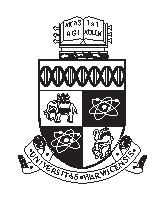
\includegraphics[width=0.4\textwidth]{crest_black.eps}
	\end{figure}
	\vspace{37mm}
	Cem Yilmaz \\
	\today
	\end{center}
	\end{titlepage}
	\tableofcontents
	\newpage
	\section{Languages}
	\subsection{Alphabet}
	\begin{tcolorbox}[colback=black!3!white,colframe=black!60!white,title=\begin{defn}Alphabet \label{Alphabet}\end{defn}]
	Alphabet is a non-empty finite set of symbols. For example,
	\begin{align}
		\Sigma_1 = \{a,b,c\} \;\;\;\;\;\;\;\;\;\;\;\;\; \Sigma_2 = \{5,8,10\}
	\end{align}
	Are alphabets which contain those symbols.
	\end{tcolorbox}
	\begin{tcolorbox}[colback=black!3!white,colframe=0black!60!white,title=\begin{defn}Language \label{Language}\end{defn}]
	Language is a potentially infinite set of finite strings over an alphabet. Using our previous alphabets, for example, we could obtain
	\begin{align}
	L_1 = \{ab,abc,aaab,ccc,ba\} \;\;\;\;\;\;\;\;\;\; L_2 = \{ a,aa,aaa,aaaa,\ldots\}
	\end{align}
	We could further define
	\begin{align}
		\Sigma^{*} = \{\text{ALL finite strings (also called words) over the alphabet }\Sigma\}
	\end{align}
	\end{tcolorbox}
	\subsection{Deterministic Final State Automata}
	
	\begin{tcolorbox}[colback=black!3!white,colframe=black!60!white,title=\begin{defn}Deterministic Finate State Automaton \label{Deterministic Finate State Automaton}\end{defn}]
	A machine $M$ defined by the tuple
	\begin{align}
	M = (Q,\Sigma,q_0,F,\delta)
	\end{align}
	is called the deterministic finite state automaton or a deterministic finite state machine. The $Q$ refers to states, $\Sigma$ to the alphabet,  $q_0$ to the initial/starting state, $F$ to the final state and $\delta$ as the state transition.
	\end{tcolorbox}
	To represent a deterministic finite state automaton, consider the following diagram:
\begin{figure}[H]
    \centering
    \incfig{dfa}
    \caption{Exemplar deterministic finite state automata state diagram}
    \label{fig:dfa}
\end{figure}
Which represents the following table of values:
\begin{table}[H]
	\centering
	\caption{State Transition Table}
	\label{tab:label}
	\begin{tabular}{|c||c|c|c|}
		\hline
		\delta & $a$ & $b$ & $c$ \\
		\hline
		\hline
		$q_0$ & $q_1$ & $q_2$ & $q_2$ \\
		\hline
		$q_1$ & $q_1$ & $q_3$ & $q_3 $ \\
		\hline
		$q_2$ & $q_2$ & $q_2$ & $q_2$ \\
		\hline
		$q_3$ & $q_3$ & $q_3$ & $ q_3$ \\
		\hline
	\end{tabular}
\end{table}
In other words, if the input string finishes at $q_1$, we accept the input. If it finishes in any other node otherwise, reject.
\begin{tcolorbox}[colback=black!3!white,colframe=black!60!white,title=\begin{defn}The Empty Word \label{The Empty Word}\end{defn}]
The length of $|\varepsilon| = 0$. The Language $L_1$ is the empty language, $L_2 = \{ \varepsilon\}$ is a non-empty language. Note that $\Sigma^{*}$ always contains $\varepsilon$. The role that of the empty string is to be a monoid in our system.
\end{tcolorbox}
\begin{tcolorbox}[colback=black!3!white,colframe=black!60!white,title=\begin{defn}Monoid \label{Monoid}\end{defn}]
Comprise of a set, an associative binary operation on the set with an identity element.
\begin{align}
	(\mathbb{N}_0, + ,0) & \text{ is a monoid. Here, $+$ denotes addition.} \\
	(\mathbb{N},\times ,1) &\text{ is a monoid. Here, $\times $ is multiplication.}\\
	(\Sigma^{*},\circ,\varepsilon) & \text{ is a monoid. Here, $\circ$ denotes string concatenation.}
\end{align}
\end{tcolorbox}
\begin{tcolorbox}[colback=black!3!white,colframe=black!60!white,title=\begin{defn}Transition Function \label{Transition Function}\end{defn}]
The transition function is denoted as
\begin{align}
\delta(q_i,\text{string}) = q_j
\end{align}k
In other words, we take a state $q_i$, a string input, and after running the string, we get output state $q_j$. Note that the string can be a single letter or a bigger string. In case of a non-letter string, sometimes the $\delta$ is denoted as $\hat{\delta}$ instead. Formally,
\begin{align}
	\hat{\delta}:Q\times \Sigma^{*} \to Q	
\end{align}
such that
\begin{align}
	&\forall q \in Q, \hat{\delta}(q,\varepsilon) = q \\
	&\forall q \in Q \land s \in \Sigma^{*} \text{ s.t. } s = wa \text{ for some } w \in \Sigma^{*} \land a \in \Sigma, \hat{\delta}(q,s) = \delta(\hat{\delta}(q,w),a)
\end{align}
\end{tcolorbox}
\begin{tcolorbox}[colback=black!3!white,colframe=black!60!white,title=\begin{defn}Language accepted by DFA \label{Language accepted by DFA}\end{defn}]
Consider a DFA $M = (Q,\Sigma,q_0,F,\delta)$. The language accepted or recognised by $M$ is denoted by $L(M)$ and is defined as
\begin{align}
L(M) = \{ s \in \Sigma^{*} | \hat{\delta}(q_0,s) \in F \}
\end{align}
\end{tcolorbox}
\begin{tcolorbox}[colback=black!3!white,colframe=black!60!white,title=\begin{defn}Run of a DFA \label{Run of a DFA}\end{defn}]
Consider a DFA  $m = (Q,\Sigma,q_0,F,\delta).$ Consider a string $s=s_1s_2\ldots s_n$, where $s_i \in \Sigma$ for each $i \in [n]$. The run of $M$ on the empty word $\varepsilon$ is just the state $q_0$. The run of $M$ on the word $s$ is a sequence of states $r_0,r_1,\ldots,r_n$, where
\begin{align}
	r_0&=q_0 \\
\forall i \in [n],r_i &= \delta(r_{i-1},s_i)
\end{align}
\end{tcolorbox}
\subsection{Languages}
\begin{tcolorbox}[colback=black!3!white,colframe=black!60!white,title=\begin{defn}Regular Language \label{Regular Language}\end{defn}]
A language $L$ is called regular if it is accepted by some deterministic finite state automata (DFA)
\end{tcolorbox}
\begin{tcolorbox}[colback=black!3!white,colframe=black!60!white,title=\begin{defn}NFA \label{NFA}\end{defn}]
Formally, the extended transition $\hat{\delta}$ for an NFA ($Q,\Sigma,q_0,F,\delta)$ is a function $\hat{\delta}: Q \times \Sigma^{*} \to \mathbb{P}(Q)$ and is defined as follows:
\begin{align}
	\forall q \in Q, \hat{\delta}(q,\varepsilon) &= ECLOSE(q) \\
\forall q \in Q \land s \in \Sigma^{*} : s&=wa \text{ for some } w \in \Sigma^{*} \land a \in \Sigma, \hat{\delta}(q,s) = ECLOSE(\cup_{q'\in \hat{\delta}(q,w)} \delta(q',a))
\end{align}
It is useful to first compute the $\varepsilon$ closure of an input and then consider the input string to see where it possible leads, repeating the process.
\end{tcolorbox}
\begin{tcolorbox}[colback=black!3!white,colframe=black!60!white,title=\begin{cor}Language of NFA \label{Language of NFA}\end{cor}]
        Consider an NFA $M = (Q,\Sigma,q_0,F,\delta)$. The run of $M$ on the word $s$ is a sequence of states $r_0,r_1,\ldots,r_n$ such that
                \begin{align}
			r_0 &= q_0 \\
			\exists s_1,s_2,\ldots,s_n \in \Sigma& \cup \{\varepsilon\} \text{ such that } s = s_1s_2\ldots s_n \land \forall i \in [n], r_i \in \delta(r_{i-1}) \in \delta(r_{i-1},s_i)
                \end{align}
\end{tcolorbox}
\subsection{Operations on Regular Languages}
\begin{tcolorbox}[colback=black!3!white,colframe=black!60!white,title=\begin{defn}Complement Language \label{Complement Language}\end{defn}]
Suppose $L$ is regular. Is $\overline{L} = \Sigma^{*}-L$ also regular? Yes. If
\begin{align}
M = (Q,\Sigma,q_0,F,\delta)
\end{align}
is a DFA for $L$ then
\begin{align}
	M'=(Q,\Sigma,q_0, Q-F, \delta)
\end{align}
is a DFA for $\overline{L}$
\end{tcolorbox}
\begin{tcolorbox}[colback=black!3!white,colframe=black!60!white,title=\begin{defn}Intersection \label{Intersection}\end{defn}]
If $L_1$ and $L_2$ are regular, then
\begin{align}
L_1 \cap L_2
\end{align}
Is also a regular language. Consider
\begin{align}
	M_1 = (Q_1,\Sigma,q_1,F_1,\delta_1) \\
	M_2=(Q_2,\Sigma,q_2,F_2,\delta_2)
\end{align}
We define $M_3$ where
\begin{align}
	M_3 = (Q,\Sigma, q, F, \delta) \\
	Q = Q_1 \times Q_2 \\
	q = (q_1,q_2) \\
	F = F_1 \times F_2
\end{align}
For every $a \in \Sigma$, $x \in Q_1$, $y\in Q_2$ we have
\begin{align}
	\delta((x,y),a) = (\delta_1(x,a),\delta_2(y,a))
\end{align}
\end{tcolorbox}
\begin{tcolorbox}[colback=black!3!white,colframe=black!60!white,title=\begin{defn}Union \label{Union}\end{defn}]
If $L_1$ and $L_2$ are regular, then
\begin{align}
L_1 \cup  L_2
\end{align}
Is also a regular language. Consider
\begin{align}
	M_1 = (Q_1,\Sigma,q_1,F_1,\delta_1) \\
	M_2=(Q_2,\Sigma,q_2,F_2,\delta_2)
\end{align}
We define $M_3$ where
\begin{align}
	M_3 = (Q,\Sigma, q, F, \delta) \\
	Q = Q_1 \times Q_2 \\
	q = (q_1,q_2) \\
	F = (F_1 \times  Q_2) \times (Q_1 \times F_2)
\end{align}
For every $a \in \Sigma$, $x \in Q_1$, $y\in Q_2$ we have
\begin{align}
	\delta((x,y),a) = (\delta_1(x,a),\delta_2(y,a))
\end{align}
\end{tcolorbox}
\begin{tcolorbox}[colback=black!3!white,colframe=black!60!white,title=\begin{defn}Subtraction \label{Subtraction}\end{defn}]
We know that
\begin{align}
L_1 - L_2 = L_1 \cap \overline{L}_2
\end{align}
Therefore it is closed from our previous proofs.
\end{tcolorbox}
\begin{tcolorbox}[colback=black!3!white,colframe=black!60!white,title=\begin{defn}Reverse \label{Reverse}\end{defn}]
Suppose $L$ is regular. Is $L^{Rev}$ also regular?
\begin{align}
L^{Rev} = \{ w | w \text{ is the reverse of some string in }L \}
\end{align}
\end{tcolorbox}
\subsection{Non-Deterministic Finite Automata (NFA)}
\begin{tcolorbox}[colback=black!3!white,colframe=black!60!white,title=\begin{defn}NFA \label{NFA}\end{defn}]
An NFA can have NONE or MULTIPLE transitions out of a state on reading the same symbol. The definition of an NFA is similar to that of a DFA, except the transition function is re-defined as follows:
\begin{align}
\delta : Q \times \left( \Sigma \cup \{\varepsilon\} \right) \to 2^{Q}
\end{align}
\end{tcolorbox}
\begin{tcolorbox}[colback=black!3!white,colframe=black!60!white,title=\begin{defn}Extended Transition Function \label{Extended Transition Function}\end{defn}]
The extended transition function is similar to that of a DFA, except it also considers $\varepsilon$ transitions. Formally,
\begin{align}
	\forall q \in Q, \hat{\delta}(q,\varepsilon) = ECLOSE(q) \\
\forall q \in Q \land s \in \Sigma^{*} : s=wa, w \in \Sigma^{*} \land a \in \Sigma, \hat{\delta}(q,s) = ECLOSE\left(\bigcup_{q'\in \hat{\delta}(q,w)}\delta(q',a)\right)
\end{align}
\end{tcolorbox}
\begin{tcolorbox}[colback=black!3!white,colframe=black!60!white,title=\begin{defn}E-closure \label{E-closure}\end{defn}]
The function $ECLOSE(q)$ denotes all states that can be reached from $q$ by following $\varepsilon$-transitions alone.
\end{tcolorbox}
\begin{tcolorbox}[colback=black!3!white,colframe=black!60!white,title=\begin{defn}Language \label{Language}\end{defn}]
Consider an NFA $M=(Q,\Sigma,q_0,F,\delta)$. The language accepted or recognised by $M$ denoted by $L(M)$ and is defined as
\begin{align}
	L(M) = \{s \in \Sigma^{*} | \hat{\delta}(q_0,s) \cap F \neq \varnothing \}
\end{align}
\end{tcolorbox}
\begin{tcolorbox}[colback=black!3!white,colframe=black!60!white,title=\begin{defn}Run of M \label{Run of M}\end{defn}]
A run of $M$ on the word $s$ is a sequence of states $r_0,r_1,\ldots,r_n$ such that
\begin{align}
r_0=q_0 \\
\exists s_1,s_2,\ldots s_n \in \Sigma \cup \{ \varepsilon \} \text{ such that } s=s_1s_2 \ldots s_n \land \forall i \in [n], r_i \in \delta(r_{i-1},s_i)
\end{align}
\end{tcolorbox}
\begin{tcolorbox}[colback=black!3!white,colframe=black!60!white,title=\begin{defn}Subset Construction \label{Subset Construction}\end{defn}]
Let $N = (Q,\Sigma, q_0,F,\delta)$ be the NFA we want determinise. Denote using $M = (Q_1,\Sigma,q_1,F_1,\delta_1)$ the target DFA. We have
\begin{align}
Q_1=2^{Q} \\
q_1 = ECLOSE(q_0)\\
F_1 = \{X \subseteq Q | X \cap F \neq \varnothing\} \\
\delta_1(X,a) = \bigcup_{x \in X} ECLOSE(\delta(x,a)) = \{ z | \text{ for some } x \in X, z \in ECLOSE(\delta(x,a))\}
\end{align}
\end{tcolorbox}
\begin{tcolorbox}[colback=black!3!white,colframe=black!60!white,title=\begin{exmp}Subset Construction \label{Subset Construction}\end{exmp}]
        \begin{figure}[H]
        	\centering
        	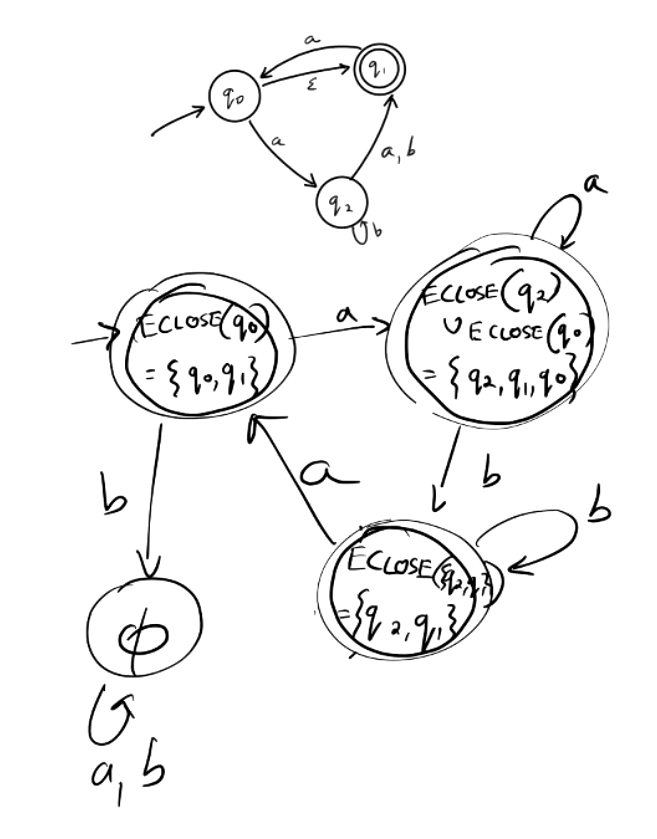
\includegraphics[width=0.8\textwidth]{one.png}
        	\caption{Subset Construction Example}
        	\label{fig:one-png}
        \end{figure}
\end{tcolorbox}
\section{Regular Expressions}
\subsection{Definition}

\begin{tcolorbox}[colback=black!3!white,colframe=black!60!white,title=\begin{defn}Regular Expression \label{Regular Expression}\end{defn}]
The language generated by a regular expression $R$ is $L(R)$ and is defined as 
\begin{align}
	L(R) &= \{a \} &\Leftarrow R&= a \text{ for some }a\in \Sigma \\
	L(R) &= \{ \varepsilon \} &\Leftarrow R &= \varepsilon \\
	L(R) &= \varnothing &\Leftarrow R &= \varnothing \\
	L(R) &= L(R_1) \cup L(R_2) &\Leftarrow R &= R_1+R_2 \\
	L(R) &= L(R_1) . L(R_2) &\Leftarrow R &= R_1 . R_2 \\ 
	L(R) &= (L(R_1))^{*} &\Leftarrow R &= R_1^{*}
\end{align}
\end{tcolorbox}
\begin{tcolorbox}[colback=black!3!white,colframe=black!60!white,title=\begin{defn}Star \label{Star}\end{defn}]
For any $S \subseteq \Sigma^{*}$, we have
\begin{align}
S^{*} = \{ \varepsilon \} \cup S \cup S^2 \cup \ldots
\end{align}
\end{tcolorbox}
\begin{tcolorbox}[colback=black!3!white,colframe=black!60!white,title=\begin{exmp}Regular Expressions \label{Regular Expressions}\end{exmp}]
        Consider $\Sigma = \{a,b\}$ and let $R = (a+b)^{*}$. What is $L(R)$?
                \begin{align}
                L(R) = \Sigma^{*}
                \end{align}
	Let $R = (a+b)^{*}(a+bb)$. What is $L(R)$?
	\begin{align}
		L(R) = \Sigma^{*} . \{a,bb\}
	\end{align}
\end{tcolorbox}
\begin{tcolorbox}[colback=black!3!white,colframe=black!60!white,title=\begin{thm}Regularity \label{Regularity}\end{thm}]
	A language is accepted by an NFA/DFA if and only if it is generated by a regular expression. Note that this also implies that NFA are regular.
\end{tcolorbox}
\subsection{Conversion to NFA}
\begin{tcolorbox}[colback=black!3!white,colframe=black!60!white,title=\begin{defn}Union / Plus \label{Union / Plus}\end{defn}]
For NFA $N_1$ expressing $R_1$ and NFA $N_2$ expressing $R_2$, their plus is
\begin{figure}[H]
	\centering
	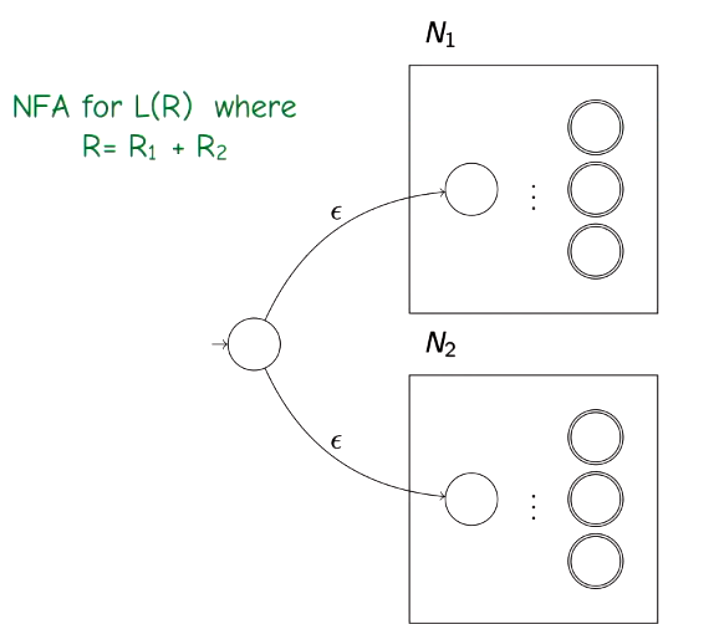
\includegraphics[width=0.5\textwidth]{two.png}
	\caption{Plus as an NFA}
	\label{fig:two-png}
\end{figure}
\end{tcolorbox}
\begin{tcolorbox}[colback=black!3!white,colframe=black!60!white,title=\begin{defn}Concat \label{Concat}\end{defn}]
\begin{figure}[H]
	\centering
	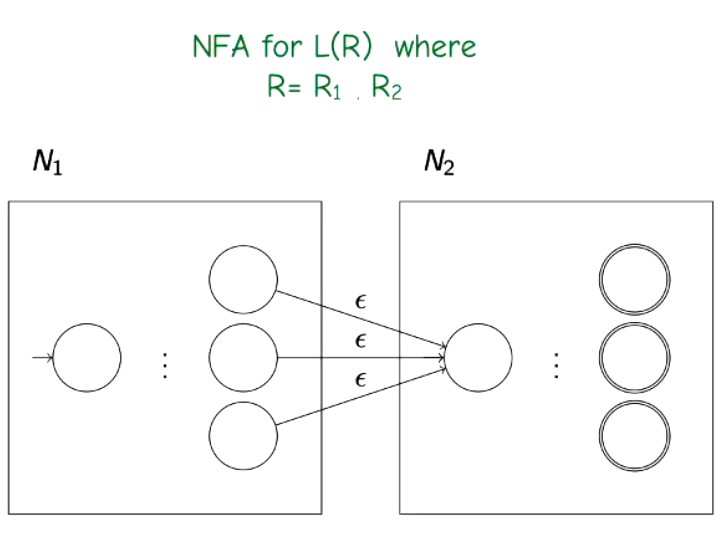
\includegraphics[width=0.5\textwidth]{three.png}
	\caption{Concat}
	\label{fig:three-png}
\end{figure}
\end{tcolorbox}
\begin{tcolorbox}[colback=black!3!white,colframe=black!60!white,title=\begin{defn}Star \label{Star}\end{defn}]
\begin{figure}[H]
	\centering
	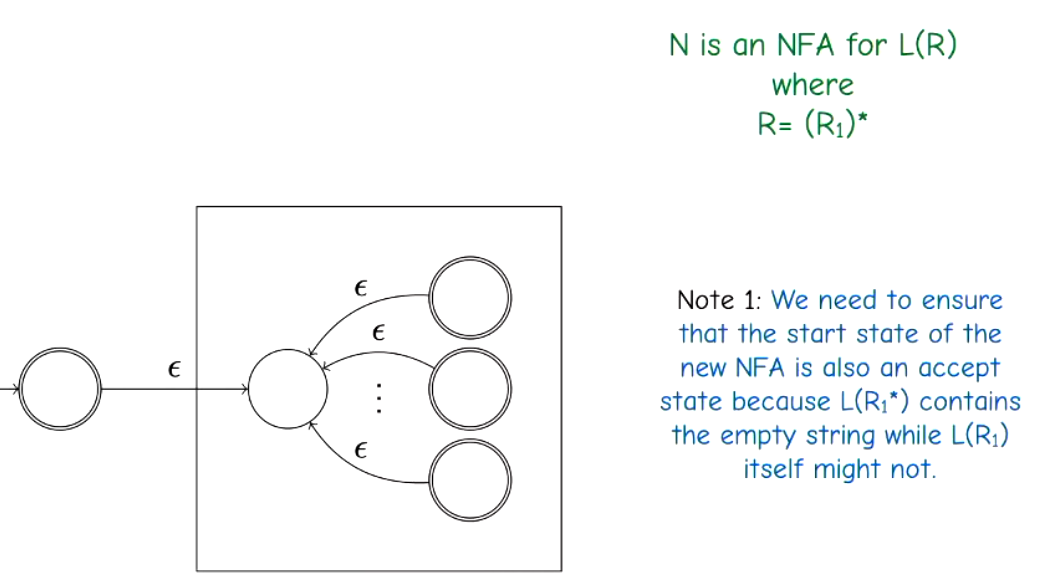
\includegraphics[width=0.8\textwidth]{four.png}
	\caption{Star as an NFA}
	\label{fig:four-png}
\end{figure}
\end{tcolorbox}
\begin{tcolorbox}[colback=black!3!white,colframe=black!60!white,title=\begin{exmp}Regular Expression to NFA \label{Regular Expression to NFA}\end{exmp}]
        \begin{figure}[H]
        	\centering
        	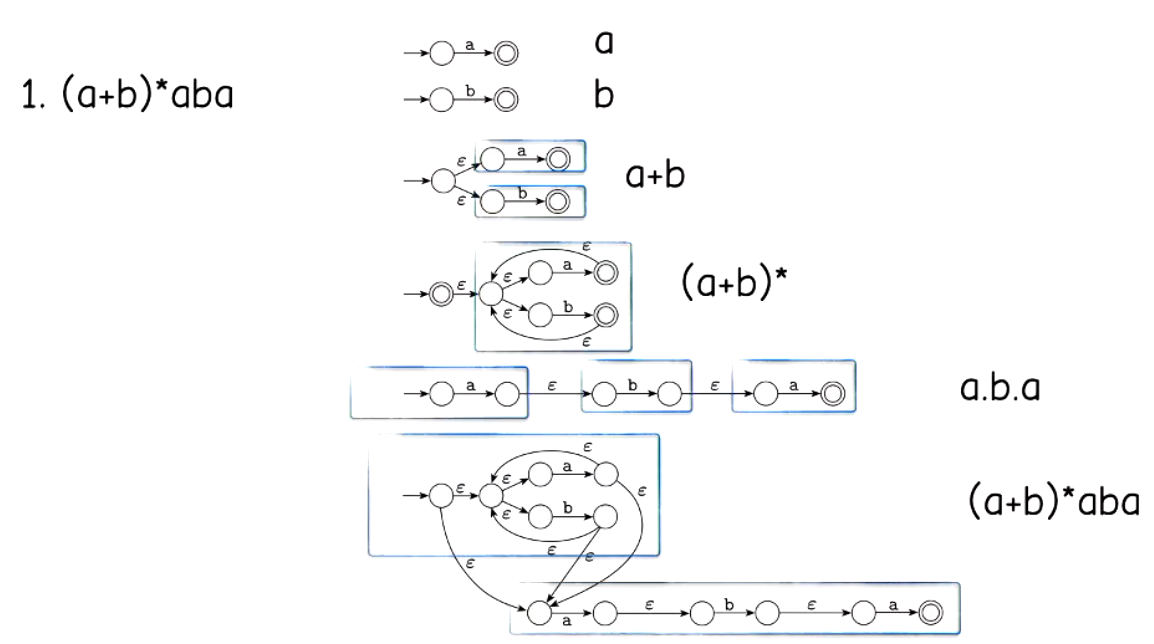
\includegraphics[width=1\textwidth]{five.png}
        	\caption{Regular Expression to NFA}
        	\label{fig:five-png}
        \end{figure}
                \begin{align}
                
                \end{align}
	\end{tcolorbox}
	\begin{tcolorbox}[colback=black!3!white,colframe=black!60!white,breakable,enhanced,title=\begin{exmp}NFA To Regular Expression \label{NFA To Regular Expression}\end{exmp}]
	Consider the NFA
	\begin{figure}[H]
		\centering
		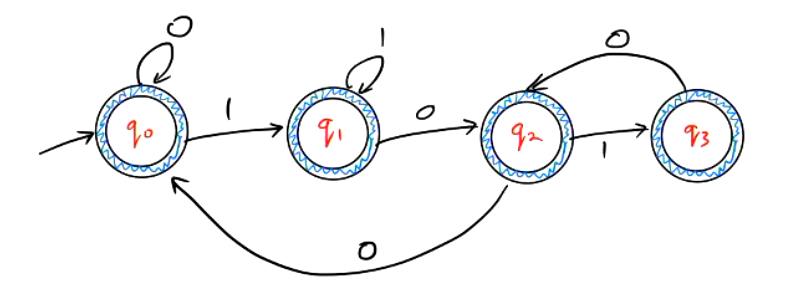
\includegraphics[width=0.8\textwidth]{six.png}
		\caption{NFA}
		\label{fig:six-png}
	\end{figure}
	\begin{figure}[H]
		\centering
		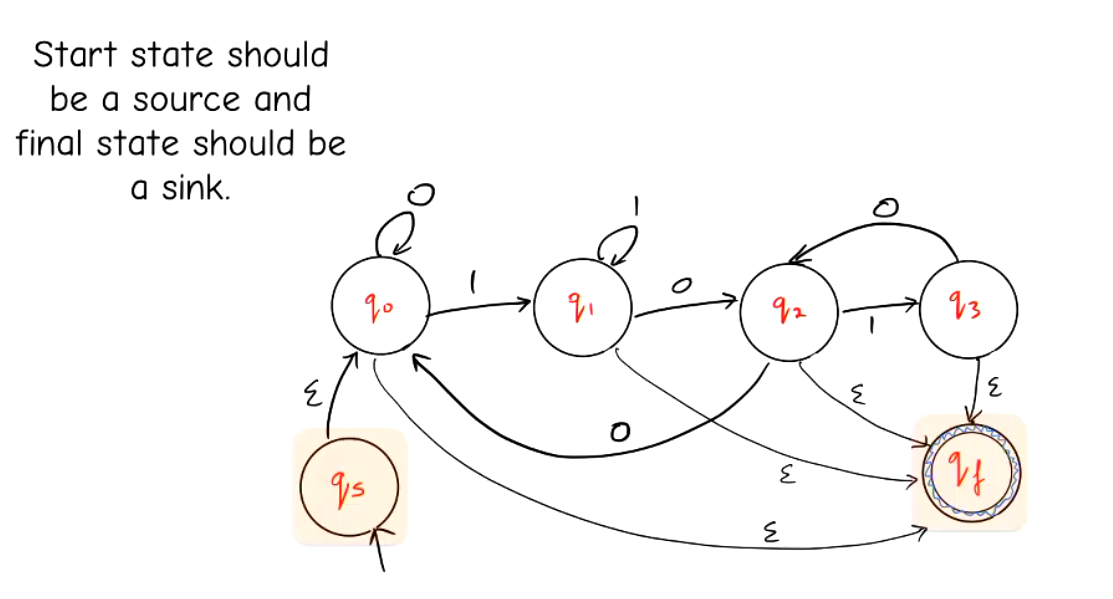
\includegraphics[width=0.8\textwidth]{seven.png}
		\caption{Sink addition}
		\label{fig:seven-png}
	\end{figure}
	\begin{figure}[H]
		\centering
		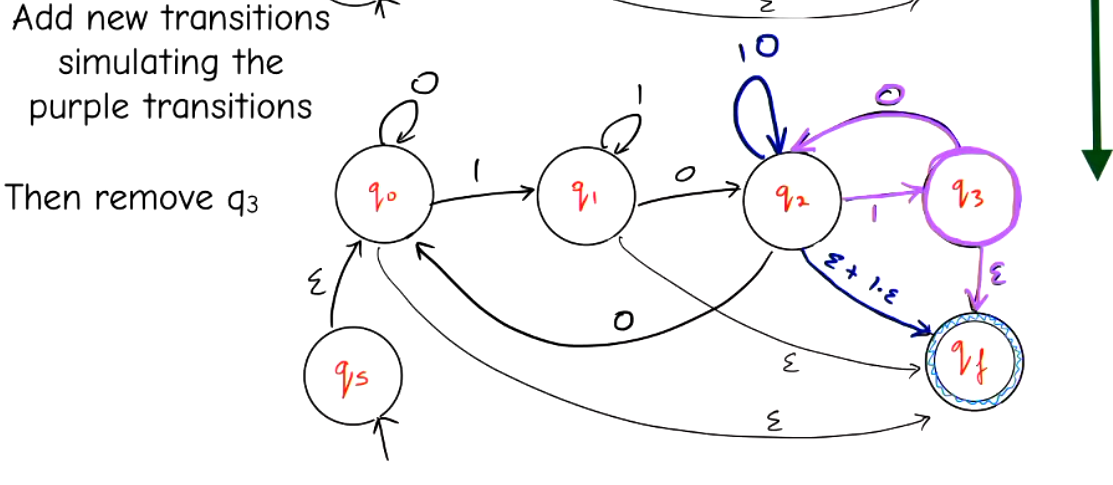
\includegraphics[width=0.8\textwidth]{eight.png}
		\caption{Re-making the transition}
		\label{fig:eight-png}
	\end{figure}	
	\begin{figure}[H]
		\centering
		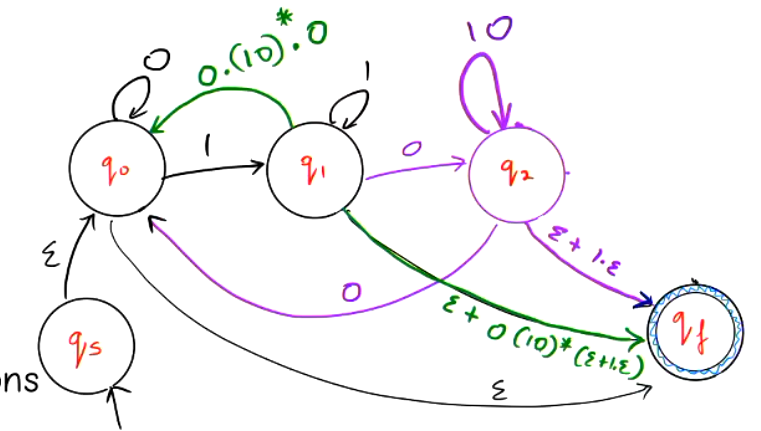
\includegraphics[width=0.8\textwidth]{nine.png}
		\caption{Removal of next node}
		\label{fig:nine-png}
	\end{figure}
	\begin{figure}[H]
		\centering
		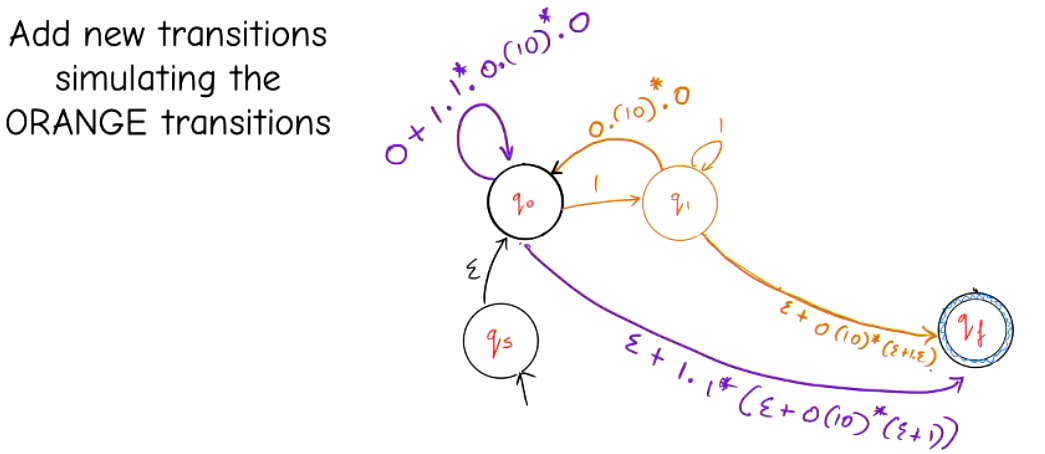
\includegraphics[width=0.8\textwidth]{ten.png}
		\caption{Another node}
		\label{fig:ten-png}
	\end{figure}
	\begin{figure}[H]
		\centering
		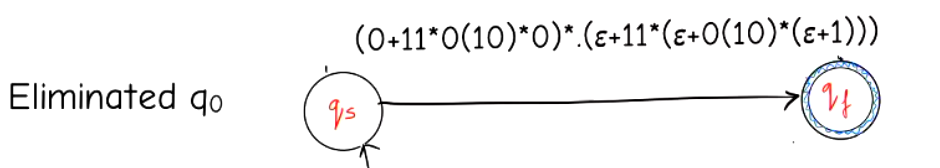
\includegraphics[width=0.8\textwidth]{eleven.png}
		\caption{Last}
		\label{fig:eleven-png}
	\end{figure}
\end{tcolorbox}
\begin{tcolorbox}[colback=black!3!white,colframe=black!60!white,title=\begin{defn}GNFA \label{GNFA}\end{defn}]
A run on GNFA on the word $s$ is a sequence of states $r_0,r_1,\ldots,r_n$ such that
\begin{align}
r_0=q_0\\
\exists s_1,s_2,\ldots,s_n \in \Sigma^{*} \text{ such that }s=s_1s_2\ldots s_n \land \forall i \in [n], s_i \in L(\delta(r_{i-1},r_i))
\end{align}
\begin{figure}[H]
	\centering
	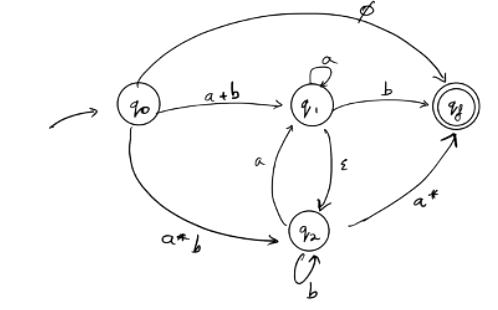
\includegraphics[width=0.8\textwidth]{twelve.png}
	\caption{Example GNFA}
	\label{fig:twelve-png}
\end{figure}
\end{tcolorbox}
\section{Proving Regularity}
\subsection{Myhill-Nerode}
\begin{tcolorbox}[colback=black!3!white,colframe=black!60!white,title=\begin{exmp}Language L \label{Language L}\end{exmp}]
        Let
                \begin{align}
                L = \{0^{n}1^{n} | n\ge 0 \}
                \end{align}
		Is $L$ regular?
\end{tcolorbox}
\begin{tcolorbox}[colback=black!3!white,colframe=black!60!white,title=\begin{defn}Distinguishability \label{Distinguishability}\end{defn}]
Strings $x$ and $y$ distinguishable by $L$ if there is a string $z$ such that $x.z \in L$ but $y.z \not\in L$ or vice-versa. If they are indistinguishable by $L$ otherwise, we write
\begin{align}
	X \equiv_L y
\end{align}
Note, $\equiv_L$ is an equivalence relation. In other words, two words are in the same equivalent class if they end in the same node.
\end{tcolorbox}
\begin{tcolorbox}[colback=black!3!white,colframe=black!60!white,title=\begin{thm}Myhill-Nerode\label{Regularity}\end{thm}]
	$L$ is a regular language if and only iff $\equiv_L$ has a finite index. This will prove that they must all lie in distinct equivalence classes of $\equiv_L$ and so $\equiv_L$ must have an infinite number of equivalence classes.
\end{tcolorbox}
\begin{tcolorbox}[colback=black!3!white,colframe=black!60!white,title=\begin{exmp}Myhill-Nerode Example \label{Myhill-Nerode Example}\end{exmp}]
        We will solve our initial example using our new theorem. Let $L = \{0^{n}1^{n} | n \ge 0 \}$ 
	\begin{enumerate}
		\item $0$ 
		\item $00$ 
		\item $000$ 
		\item $\vdots$
		\item $0^{r}$
	\end{enumerate}
	We show that each $0$ belongs to a different equivalence class. Consider concatenating $1$ into every end of $ 0$. This means that the first string is distinguishable. Consider concatenating  $11$ now. Second is distinguishable, but rest is not. Following this logic for every $0$, from our theorem, we know that each $0$ must belong to an unique state, therefore, it is an infinite DFA with infinite number of nodes, meaning it is not regular.
\end{tcolorbox}
\begin{tcolorbox}[colback=black!3!white,colframe=black!60!white,title=\begin{exmp}Myhill-Nerode Example Two \label{Myhill-Nerode Example Two}\end{exmp}]
        Prove that the language
                \begin{align}
                \{a^{n}b^{n}c^{n} | n\ge 0 \}	
                \end{align}
	over $\{a,b,c\}$ is not regular.
	\begin{proof}
		By Myhill-Nerode/index of the language. Consider the infintie set of strings generated by $a^{*}$. For any $a^{i}$, $a^{j}$ where $i \neq j$, observe that $a^{i}\cdot a^{m-i} b^{m}c^{m}=a^{m}b^{m}c^{m}$, which is in $L$, while $a^{j}\cdot a^{m-i}b^{m}c^{m} \not\in L$. This implies that the set of strings generated by $a^{*}$ is pairwise distinguishable by $L$, and so $L$ has an infinite index, implying that $L$ must be non-regular.
	\end{proof}
\end{tcolorbox}
\begin{tcolorbox}[colback=black!3!white,colframe=black!60!white,title=\begin{exmp}Myhill-Nerode Example Three \label{Myhill-Nerode Example Three}\end{exmp}]
        Prove that the language
                \begin{align}
                L= \{1^{n} | n \text{ is prime} \}	
                \end{align}
		over $\{1\}$ is not regular.
		\begin{proof}
			We claim that $1^{i}$ is distinguishable from $1^{j}$ for every distinct $i,j$. Assume without loss of generality that $i<j$. Pick an arbitrary prime $p>i$, where $p>2$. Since $p>2$ and $j-i > 0$, we know that $p + 0(j-i)$ is prime and $p+p(j-i)$ is not prime. Walking down this list, at some point a prime will switch to a none prime. Let $k \le p$ be the first such point. We now have that $p+(k-1)(j-i)$ is prime. We show that
			\begin{align}
				1^{i}.1^{[p+(k-1)(j-i)]-i} \in L \\
				1^{j}.1^{[p+(k-1)(j-i)]-i}\not\in L
			\end{align}
		\end{proof}
\end{tcolorbox}
\subsection{Pumping Lemma}
\begin{tcolorbox}[colback=black!3!white,colframe=black!60!white,title=\begin{defn}Intuition\label{Pumping Lemma}\end{defn}]
If there is a cycle that is reachable from the start state and which can reach an accept state, in the state diagram of the DFA $M$, then $L(M)$ is infinite. In fact this is an iff statement. Furthermore, this is equivalent to saying that $L(M)$ accepts words more than the number of states it has.
\end{tcolorbox}
\begin{tcolorbox}[colback=black!3!white,colframe=black!60!white,title=\begin{defn}Pumping Lemma \label{Pumping Lemma}\end{defn}]
If $L$ is a regular language, then $\exists  m>0$ such that $\forall  w \in L : |w| > m$, $\exists $ a decomposition $w=xyz : |y|>0, |xy|<m$ such that $\forall  i\ge 0, xy^{i}z \in L$
\begin{proof}
	Let $M = (Q,\Sigma, q_0, F, \delta)$ be a DFA accepting $L$. Let us set
	\begin{align}
		m = |Q|
	\end{align}
	Consider any $w \in L : |w| \ge m$. Consider the run of $w$ on $M$. (If $w$ does not exist, this statement is vacuously true). Let the run of $w$ on $M$ be denoted by $(\alpha_0,\alpha_1,\ldots,\alpha_{|w|})$, where $\alpha_0 = q_0$, $\alpha_{|w|} \in F$ and $\forall  j \in \{0,\ldots,|w|\}$, $\alpha_j \in Q$. By pigeon-hole principle, $\exists j_1,j_2 : j_1<j_2$ and $\alpha_{j_1}=\alpha_{j_2}$. By our choice of $j_1$, either $j_1=0$ or the partial run $(\alpha_0,\ldots,\alpha_{j_1})$ has no repeating states. Therefore, $j_1 \le |Q|$. Moreover, the partial run $(\alpha_{j_1},\ldots,\alpha_{j_2})$ is a loop in the state-transition diagram of $M$. We define
	\begin{itemize}
		\item $x$ to be the substring of $w$ consumed by $M$ in the partial run $(\alpha_0,\ldots,\alpha_j)$
		\item $y$ to be the substring of $w$ consumed by $M$ in the partial run $(\alpha_{j_1},\ldots,\alpha_{j_2})$ 
		\item $z$ to be the substring of $w$ such that $w = xyz$
	\end{itemize}
	We remain to prove that $\forall  i\ge 0, xy^{i}z \in L$. But this is true since $\forall  i\ge 0$, the run $(\alpha_0,\ldots,\alpha_{j_1}) \cdot(\alpha_{j_1},\ldots,\alpha_{j_2})^{i}\cdot(\alpha_{j_2},\ldots,\alpha_{|w|})$ is an accepting run in $M$.
\end{proof}
\end{tcolorbox}
\begin{tcolorbox}[colback=black!3!white,colframe=black!60!white,title=\begin{defn}Steps for showing non-regularity \label{Steps for showing non-regularity}\end{defn}]
\begin{enumerate}
	\item Suppose $L$ is a regular and let $m$ be the pumping length of $L$ 
	\item Choose a string $w \in L$ such that $|w| \ge m$ 
	\item Let $w = x.y.z$ be an arbitrary decomposition of $w$ such that $|xy|\le m$, $|y|>0$ 
	\item Carefully pick an integer $i$ and argue that $x.y^{i}.z \not\in L$
\end{enumerate}
\end{tcolorbox}
\begin{tcolorbox}[colback=black!3!white,colframe=black!60!white,title=\begin{exmp}Pumping Lemma Example \label{Pumping Lemma Example}\end{exmp}]
        Show that the language
                \begin{align}
                L = \{w \in \{a,b\}^{*} | n_a(w)<_b(w) \}
                \end{align}
		Is not regular.
		\begin{proof}
			Let $m$ denote the pumping length of $L$. Let us choose $w = a^{m}b^{m+1}$. Let $w=x.y.z$ be an arbitrary decomposition of $w$ such that $|xy|\le m, |y|>0$. Consider $x=a^{\alpha}, y=a^{\beta},z=a^{\gamma}b^{m+1}$ where $\beta \ge 1$ and $\alpha+\beta+\gamma = m$. Let us choose $i=2$. We have that $\alpha+2\beta+\gamma \ge \alpha + \beta + \gamma +1 = m+1$ and this is not in $L$.
		\end{proof}
\end{tcolorbox}
\begin{tcolorbox}[colback=black!3!white,colframe=black!60!white,title=\begin{exmp}Pumping Lemma Example Two \label{Pumping Lemma Example Two}\end{exmp}]
Show that the language
\begin{align}
	L = \{ w\in\{0,1\}^{*} | n_0(w) = n_1(w)\}
\end{align}
Is not regular.
\begin{proof}
        Let $m$ denote the pumping length of $L$. Let us choose $w=0^{m}1^{m}$. Then, consider the breakdown $w=x.y.z$ where $|xy| \le m$ and $y > 0$. In particular, let $x=0^{\alpha},y=0^{\beta},0^{\gamma}1^{m}$ where $\alpha+\beta+\gamma = m$ and $\beta \ge 1$. Let us choose $i=2$. We have that $\alpha+2\beta+\gamma \ge m+1$. However, $m+1 \neq m$ therefore this is not in $L$.
\end{proof}
\end{tcolorbox}
\begin{tcolorbox}[colback=black!3!white,colframe=black!60!white,title=\begin{exmp}Pumping Lemma Example 3 \label{Pumping Lemma Example 3}\end{exmp}]
        Show that the language
                \begin{align}
                \{a^{n}b^{n}c^{n} | n\ge 0 \}
                \end{align}
	over $\{a,b,c\}$ is not regular
	\begin{proof}
		By the pumping lemma. Let $L$ denote this language and for a contradiction suppose that $L$ is regular and let $m$ be its pumping length. Let $w = a^{m}b^{m}c^{m}$ and let $w=xyz$ where $|xy|\le m$ and $y>0$. Then, let $x = a^{\alpha},y=a^{\beta},z=a^{\gamma}b^{m}c^{m}$ for some $\alpha,\beta,\gamma$ where $\alpha+\beta+\gamma =m$ and $\beta >0$. Observe that $a^{\alpha+\gamma} b^{m}c^{m}}$, where $\alpha+\gamma<m$, implying that $xy^{0}z \not\in L$, a contradiction to the pumping lemma. This proves that $L$ is not regular.
	\end{proof}
\end{tcolorbox}
\section{Grammars}
\subsection{Definition}
\begin{tcolorbox}[colback=black!3!white,colframe=black!60!white,title=\begin{defn}Grammar \label{Grammar}\end{defn}]
The formal definition of a grammar is given by
\begin{align}
G = (V,\Sigma,R,S)
\end{align}
Where $V$ is the finite set of variables, $\Sigma$ is the finite alphabet, $R $ is the finite set of production rules or productions and $S \in V$ is the START variable.
\end{tcolorbox}
\begin{tcolorbox}[colback=black!3!white,colframe=black!60!white,title=\begin{exmp}Grammar Example \label{Grammar Example}\end{exmp}]
        Consider the grammar $G$
                \begin{align}
			G &= (\{S\},\{0,1\},R,S) \\
			R&: S \to {}_0S_1 \\
		   &: S \to \varepsilon
                \end{align}
		Therefore we have
		\begin{align}
			S \implies {}_0S_1 \implies {}_{00}S_{11} \implies {}_{000}S_{111} \implies 000111
		\end{align}
\end{tcolorbox}
\begin{tcolorbox}[colback=black!3!white,colframe=black!60!white,title=\begin{defn}Left-most Derivation \label{Left-most Derivation}\end{defn}]
The left-most derivation of some grammar $G$ means that you keep replacing the left-most variable.
\end{tcolorbox}
\begin{tcolorbox}[colback=black!3!white,colframe=black!60!white,title=\begin{defn}Parse Tree \label{Parse Tree}\end{defn}]
\begin{figure}[H]
	\centering
	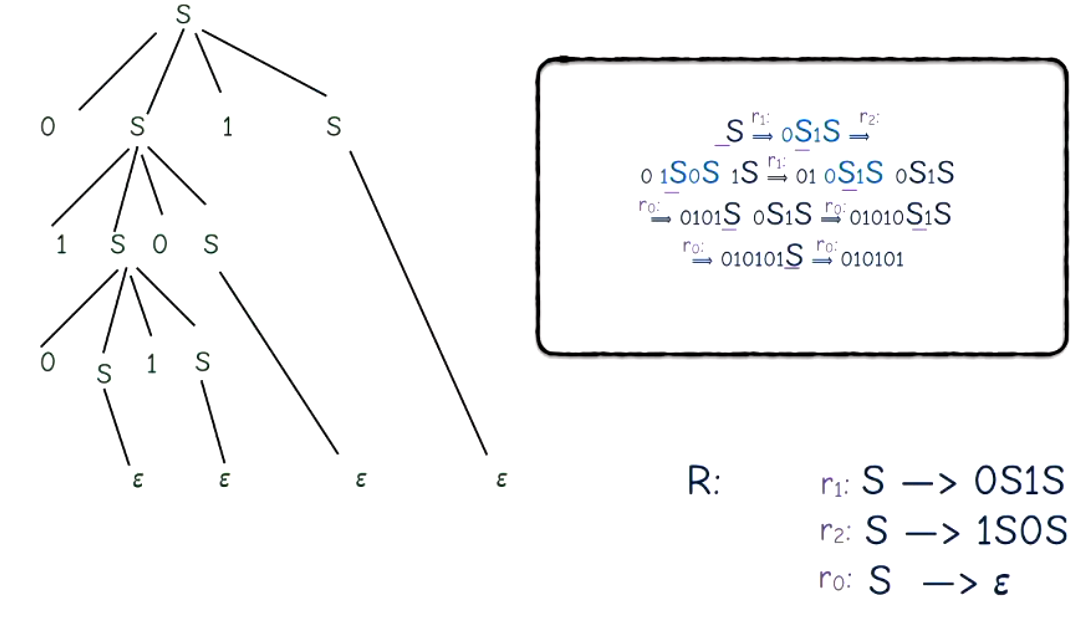
\includegraphics[width=0.8\textwidth]{thirteen.png}
	\caption{Parse Tree}
	\label{fig:thirteen-png}
\end{figure}
\end{tcolorbox}
\begin{tcolorbox}[colback=black!3!white,colframe=black!60!white,title=\begin{defn}Ambiguity \label{Ambiguity}\end{defn}]
A grammar $G$ is ambiguous if it can generate the same string with multiple parse trees if and only if the same string can be derived with two left-most derivations. Some but not all ambiguous grammars can be re-written with rules in order to get rid of the ambiguity. 
\end{tcolorbox}
\begin{tcolorbox}[colback=black!3!white,colframe=black!60!white,title=\begin{defn}Chomsky hierarchy of Grammars \label{Chomsky hierarchy of Grammars}\end{defn}]
\begin{enumerate}
	\item Regular grammars - follow the rules of $A \to xB, A\to x$ or $A \to Bx, A\to x$
	\item Context free grammars - $A \to w$ (letter) and $B$ can be anything
	\item Context sensitive - $\alpha A \gamma \to \alpha \beta \gamma$
	\item Recursively enumerable - $\alpha \to \beta$
\end{enumerate}
\end{tcolorbox} 
\subsection{Grammars and DFAs}
\begin{tcolorbox}[colback=black!3!white,colframe=black!60!white,title=\begin{exmp}DFA to right-linear Grammar \label{DFA to right-linear Grammar}\end{exmp}]
Consider the DFA 
\begin{figure}[H]
	\centering
	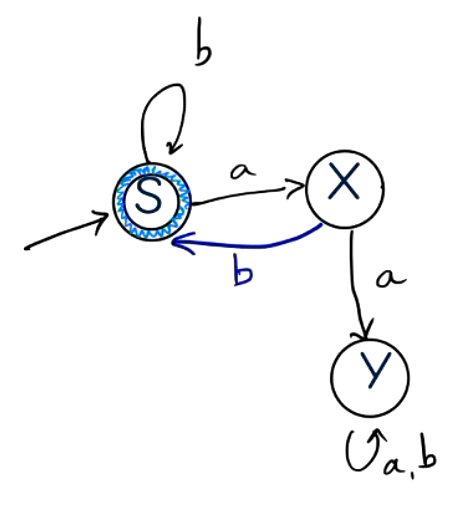
\includegraphics[width=0.22\textwidth]{fourteen.png}
	\caption{DFA}
	\label{fig:DFA}
\end{figure}
and the grammar
\begin{align}
	G = (\{S,X,Y\},\{a,b\},R,S)
\end{align}
We now write the rules according to the nodes of our DFA, that is
\begin{align}
	S &\to b.S | a.X | \varepsilon \\
	X &\to b.S | a.Y \\
	Y &\to a.Y | b.Y
\end{align}
\end{tcolorbox}
\begin{tcolorbox}[colback=black!3!white,colframe=black!60!white,title=\begin{defn}DFA to left-linera Grammar \label{DFA to left-linera Grammar}\end{defn}]
For left linear grammars, instead of starting at the beginning state, we begin at the finish state. Instead of focusing on the nodes where it goes to, we care about the nodes that lead to our finish state from the start state and repeat the process.
\end{tcolorbox}
\section{Push Down Automaton}
\begin{tcolorbox}[colback=black!3!white,colframe=black!60!white,title=\begin{defn}Push Down Automaton \label{Push Down Automaton}\end{defn}]
A push down automaton is a $6$-tuple $(Q,\Sigma,\Gamma,\delta,q_0,F)$, where $Q,\Sigma,\Gamma$ and $F$ are all finite sets and 
\begin{enumerate}
	\item $Q$ is the set of states
	\item $\Sigma$ is the input alphabet
	\item $\Gamma$ is the stack alphabet (Usually includes $\Sigma$ and $\$$ the empty stack symbol)
	\item $\delta : Q \times \Sigma_{\varepsilon} \times \Gamma_{\varepsilon} \to \mathcal{P}(Q \times $
	\item $q_0 \in Q$ is the start state
	\item $F \subseteq Q$ is the set of accept states
\end{enumerate}
Note that push down machines are non-deterministic.
\end{tcolorbox}
\begin{tcolorbox}[colback=black!3!white,colframe=black!60!white,title=\begin{defn}Transitions in PDM \label{Transitions in PDM}\end{defn}]
\begin{figure}[H]
	\centering
	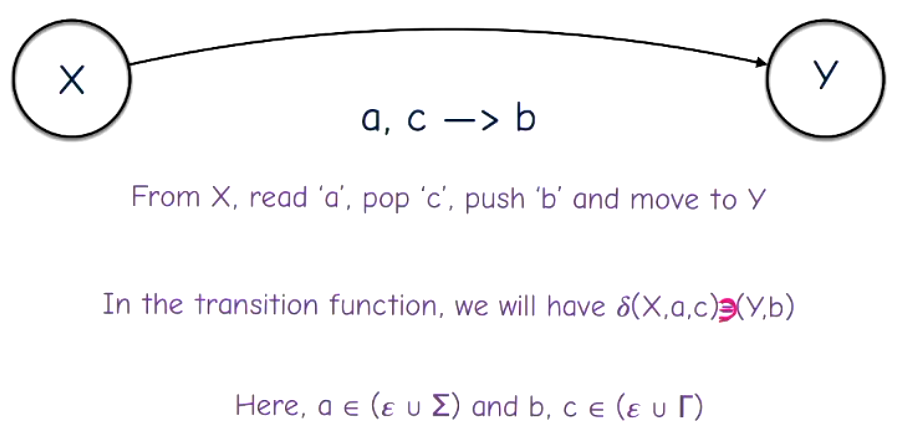
\includegraphics[width=0.8\textwidth]{fifteen.png}
	\caption{Push Down Transitions}
	\label{fig:fifteen-png}
\end{figure}
When pushing in strings, we push the last letter first so the pop can work properly.
\end{tcolorbox}
\begin{tcolorbox}[colback=black!3!white,colframe=black!60!white,title=\begin{thm}Acceptance \label{Acceptance}\end{thm}]
	Pushdown Automata accept precisely the set of Context Free Languages
\end{tcolorbox}
\subsection{CFG to PDA}
\begin{tcolorbox}[colback=black!3!white,colframe=black!60!white,title=\begin{defn}CFG to PDA \label{CFG to PDA}\end{defn}]
The following construction of a PDA from a given CFG will rely on the following three states
\begin{itemize}
	\item Start state $q_s$ 
	\item Loop state $q_I$ 
	\item Accept state $q_a$
\end{itemize}
In addition, we will implicitly use a number of auxiliary states whenever we take advantage of the shorthand notation for multiple pushes
\end{tcolorbox}
\begin{tcolorbox}[colback=black!3!white,colframe=black!60!white,title=\begin{exmp}CFG to PDA example \label{}\end{exmp}]
        \begin{figure}[H]
        	\centering
        	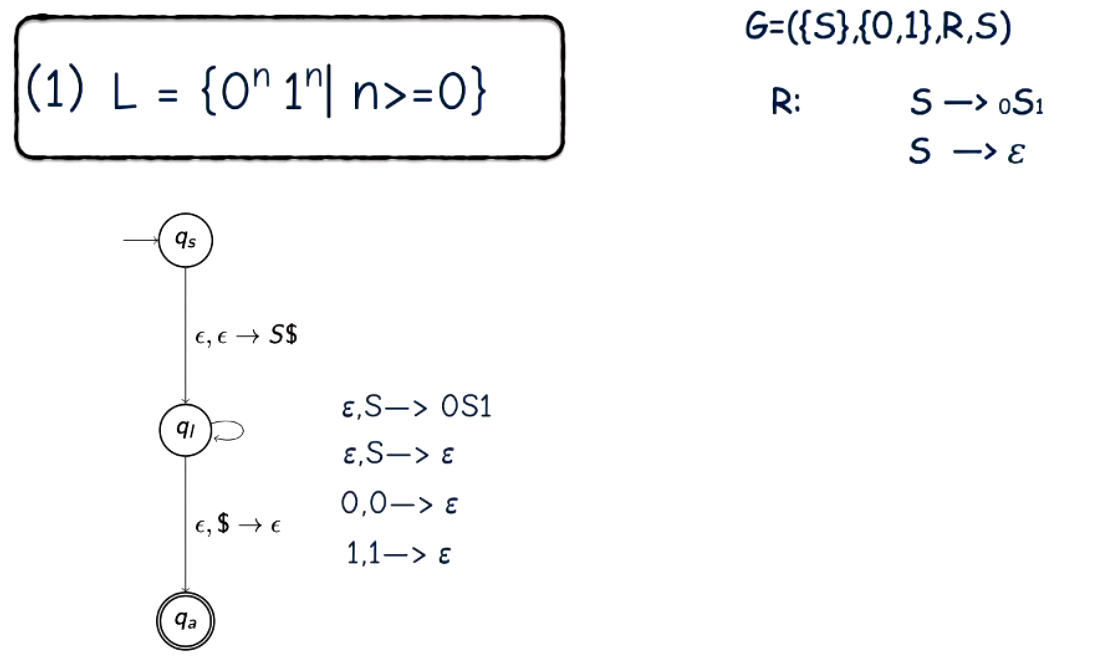
\includegraphics[width=0.8\textwidth]{sixteen.png}
        	\caption{CFG to PDA}
        	\label{CFG}
        \end{figure}
\end{tcolorbox}
\subsection{PDA to CFG}
In order to convert a PDA to a CFG, we first need to normalise it.
\begin{tcolorbox}[colback=black!3!white,colframe=black!60!white,title=\begin{defn}Normalised PDA \label{Normalised PDA}\end{defn}]
A normalised PDA has
\begin{enumerate}
	\item It has a single accept, $q_{accept}$
	\item It empties its stack before accepting
	\item Each transition either pushes a symbol onto the stack (a push move) or pops one off the stack (a pop move), but it does not do both at the same time.
\end{enumerate}
\end{tcolorbox}
\begin{tcolorbox}[colback=black!3!white,colframe=black!60!white,title=\begin{defn}A \label{A}\end{defn}]
There is a non-terminal $A_{pq}$ for each pair of states $p$ and $q$. $A_{pq}$ generates all strings which take us from state $p$ (with empty stack) to state $q$ (with empty stack). Languages accepted by the PDA is the set of strings which can be derived from the non-terminal $A_{q-initial, q-final}$
\end{tcolorbox}
\begin{tcolorbox}[colback=black!3!white,colframe=black!60!white,title=\begin{defn}Three Rules \label{Three Rules}\end{defn}]
\begin{enumerate}
	\item For each $p,q,r,s \in Q$, $u \in \Gamma$, and $a,b \in \Sigma_{\varepsilon}$ if $\delta(p,a,\varepsilon)$ contains $(r,u)$ and $\delta(s,b,u)$ contains $(q,\varepsilon)$, put the rule $A_{pq} \to aA_{rs}b$ in $G$.
	\item For each $p,q,r \in Q$, put the rule $A_{pq} \to A_{pr}A_{rq}$ in $G$ 
	\item Finally, for each $p \in Q$, put the rule $A_{pp} \to \varepsilon$ in $G$
\end{enumerate}
\end{tcolorbox}
\subsection{String in Grammar}
\begin{tcolorbox}[colback=black!3!white,colframe=black!60!white,title=\begin{defn}Cocke-Younger-Kasami \label{Cocke-Younger-Kasami}\end{defn}]
A grammar $G=(V,\Sigma,R,S)$ is in Chomsky Normal Form if every production has one of the following shapes:
\begin{enumerate}
	\item $S \to \varepsilon$ 
	\item $A \to x (x \in \Sigma \text{ is a terminal})$
	\item $A \to BC (B,C\in V\text{ where } B,C \neq S)$
\end{enumerate}
\end{tcolorbox}
\begin{tcolorbox}[colback=black!3!white,colframe=black!60!white,title=\begin{exmp}CYK Algorithm \label{CYK Algorithm}\end{exmp}]
\begin{figure}[H]
	\centering
	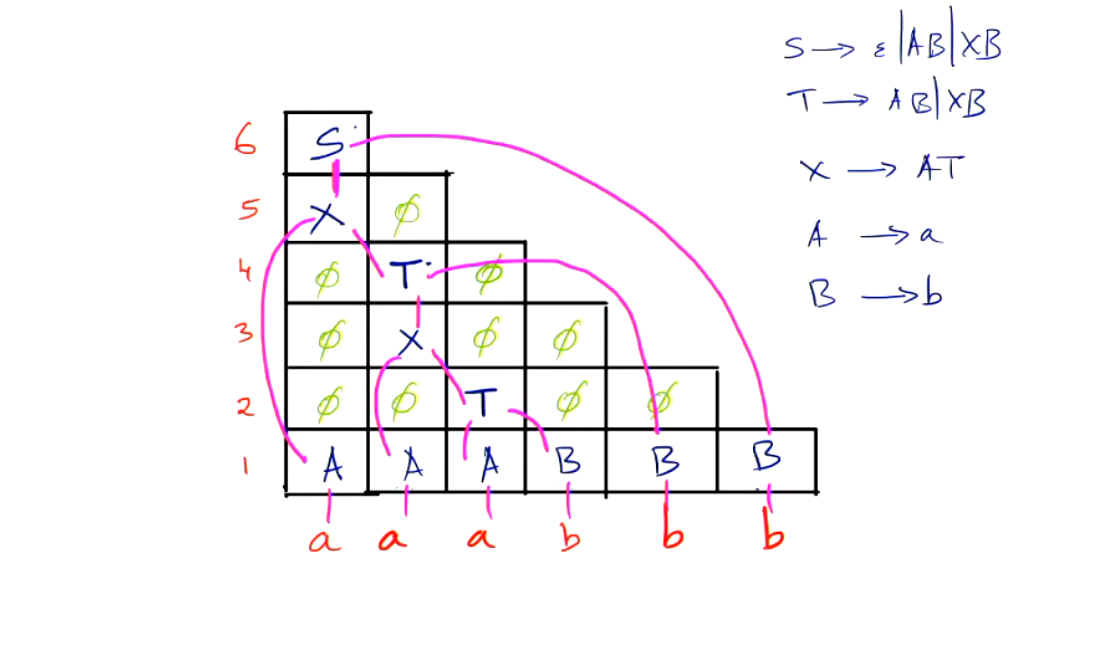
\includegraphics[width=0.8\textwidth]{seventeen.png}
	\caption{CYK Algorithm}
	\label{fig:seventeen-png}
\end{figure}
\end{tcolorbox}
\begin{tcolorbox}[colback=black!3!white,colframe=black!60!white,title=\begin{defn}To Chomsky Normal Form \label{To Chomsky Normal Form}\end{defn}]
\begin{enumerate}
	\item Create a new start variable $S_0$ and add $S_0 \to S$ 
	\item Eliminate $A \to \varepsilon$ productions where $A \neq S$ 
	\item Eliminate unit productions  $A\to B$ 
	\item Add new variables and productions to eliminate remaining violations in the rules of the form $A \to u$ where $|u| > 2$ and in rules of the form $A\to xy$ where $x$ and $y$ are both terminals
\end{enumerate}
The CYK algorithm can be used to perform a bottom up parsing of strings in polynomial time. Every string of length $n$ can be derived in exactly $2n-1$ steps
\end{tcolorbox}
\begin{tcolorbox}[colback=black!3!white,colframe=black!60!white,title=\begin{defn}Useless \label{Useless}\end{defn}]
A grammar $G$ can be called useless if it generates something that can fail to generate a string
\begin{enumerate}
	\item Find and mark all variables with a terminal or $\varepsilon$ on the right hand side
	\item Repeat until on new variables get marked
	\item If $S$ is unmarked, return $L(G)$ is empty, else return $L(G)$ is none-empty
\end{enumerate}
\end{tcolorbox}
\subsection{Pumping Lemma for CFL}
\begin{tcolorbox}[colback=black!3!white,colframe=black!60!white,title=\begin{defn}Pumping Lemma for CFL \label{Pumping Lemma for CFL}\end{defn}]
If $L$ is a CFL, then $\exists m>0$ such that $\forall w \in L : |w| \ge m, \exists $ a decomposition $w=uvxyz : |vy|>0,|vxy|\le m, \forall  i \ge 0, uv^{i}xy^{i}z \in L$
\end{tcolorbox}
\begin{tcolorbox}[colback=black!3!white,colframe=black!60!white,title=\begin{defn}Main Idea \label{Main Idea}\end{defn}]
If the length of the longest string in the right hand side of any production rule in $R$ is $b$, then any node in any parse tree yielding a string in $L(G)$ has at most $b$ children. \\
If every node of a rooted tree has at most $b$ children and the height of the tree is $h$, then the number of leaves is at most $b^{h}$. \\

\end{tcolorbox}
\begin{tcolorbox}[colback=black!3!white,colframe=black!60!white,title=\begin{defn}Using Lemma to show it is not CFL \label{Using Lemma to show it is not CFL}\end{defn}]
\begin{enumerate}
	\item Assume that $L$ is a CFL.
	\item Let $m$ be the pumping length given by the pumping lemma
	\item Choose a string $w \in L$ such that $|w|\ge m$ 
	\item Take an arbitrary decomposition  $w=uvxyz$ where $|vxy|\le m$ and $|vy|>0$ 
	\item Carefully choose an $i$ such that $uv^{i}xy^{i}z \not\in L$, contradicting the pumping lemma
\end{enumerate}
\end{tcolorbox}
\begin{tcolorbox}[colback=black!3!white,colframe=black!60!white,title=\begin{exmp}CFL Pumping Example \label{CFL Pumping Example}\end{exmp}]
        Prove that the statement
                \begin{align}
                L = \{a^{n}b^{n}c^{n} | n\ge 0 \}
                \end{align}
	Is not a CFL.
	\begin{proof}
		Assume that $L$ is a CFL. Let $m$ be the pumping length given by the pumping lemma. We choose the string $n=m$ and clearly, $|w| \ge m$.
		There are multiple cases. Consider when $vxy$ is equal to only the $a$, $b$ or $c$, i.e., only $aaaaa\ldots$ or $bbbbb\ldots$ etc. In each of these three cases, $uv^{0}xy^{0}z \not\in L$ so we just take $i=0$. For the cases where  $cxy$ is between $a$ and $b$ or $b$ and $c$, we can just take $i=0$ again. In the case where $vxy$ spans all letters, this cannot possibly be true because it is then bigger than $m$. 
	\end{proof}
\end{tcolorbox}
\begin{tcolorbox}[colback=black!3!white,colframe=black!60!white,title=\begin{defn}Properties \label{Properties}\end{defn}]
CFLs are closed under
\begin{itemize}
	\item Union
	\item Concatenation
	\item Kleene Closure
\end{itemize}
\end{tcolorbox}
\section{Turing Machines}
\subsection{Definition}
\begin{tcolorbox}[colback=black!3!white,colframe=black!60!white,title=\begin{defn}Turing Machine \label{Turing Machine}\end{defn}]
A Turing machine is a $7$-tuple, $(Q,\Sigma,\Gamma,\delta,q_0,q_{accept},q_{reject}\}$
\begin{enumerate}
	\item $Q$ is the set of states
	\item $\Sigma$ is the input alphabet not containing the blank symbol \textvisiblespace 
	\item $\Gamma$ is the tape alphabet, where \textvisiblespace $\in \Gamma$ and $\Sigma \subseteq \Gamma$ 
	\item $\delta : Q \times \Gamma \to Q \times \Gamma \times \{L,R\}$ is the transition function
	\item $q_0 \in Q$ is the start state
	\item $q_{accept}$ is the accept state and
	\item $q_{reject}$ is the reject state, where $q_{accept} \neq q_{reject}$
\end{enumerate}
\end{tcolorbox}
\begin{tcolorbox}[colback=black!3!white,colframe=black!60!white,title=\begin{defn}Configurations \label{Configurations}\end{defn}]
The configuration is given by
\begin{align}
X = (u,q,v)
\end{align}
which is a configuration if current state is $q$, the tape contains the string $uv$ and the reading head is on the first symbol of $v$. The configuration $X=(u,q,v)$ yields configuration $Y=(u',p,v')$ if the turing machine can legally go from $X$ to $Y$ in one step
\end{tcolorbox}
\begin{tcolorbox}[colback=black!3!white,colframe=black!60!white,title=\begin{defn}Decidability \label{Decidability}\end{defn}]
A language $L$ is Turing decidable if it is the language accepted by some dicider or total Turing machine. Note that Turing decidable $=$ Recursive $=$ Deciders
\end{tcolorbox}
\subsection{Decidability}
\begin{tcolorbox}[colback=black!3!white,colframe=black!60!white,title=\begin{defn}Halting Problem \label{Halting Problem}\end{defn}]
The halting problem is defined as
\begin{align}
HP := \{ <M,x> |M \text{ halts on }x \}
\end{align}
The halting problem is Turing recognisable but not decidable. 
\end{tcolorbox}
\begin{tcolorbox}[colback=black!3!white,colframe=black!60!white,title=\begin{defn}Membership Problem \label{Membership Proble}\end{defn}]
The membership problem is defined as
\begin{align}
MP := \{ <M,x> | x \in L(M)\}
\end{align}
It is also Turing recognisable but not decidable. We construct a new machine $M'$ obtained from $M$ as follows
\begin{itemize}
	\item Add a new accept state to $M$ 
	\item Make all incoming transitions to the old accept and reject states go to the new accept state
\end{itemize}
Simulate the assumed decider $N$ on input $<M',x>$ and accept if and only if $N$ accepts.
\begin{figure}[H]
	\centering
	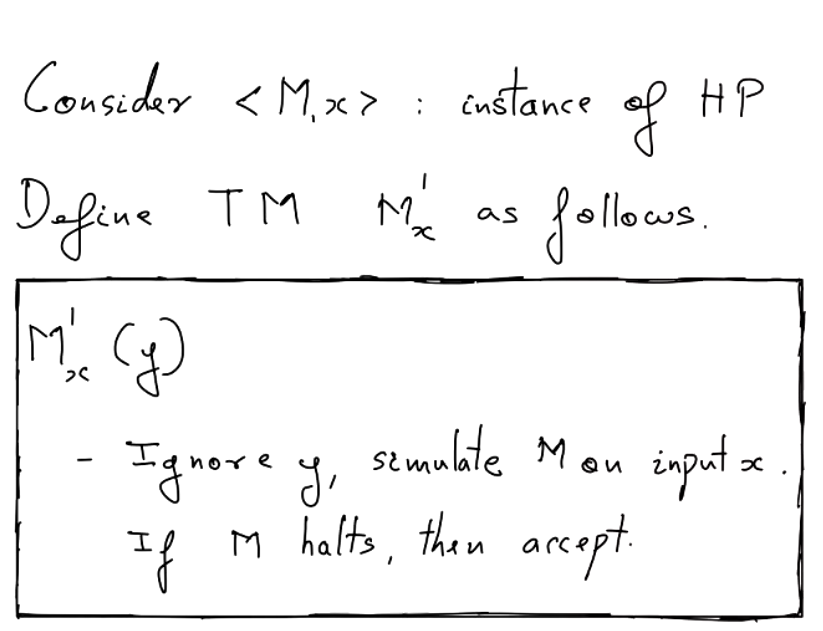
\includegraphics[width=0.6 \textwidth]{nineteen.png}
	\caption{HP to MP}
	\label{fig:nineteen-png}
\end{figure}
\end{tcolorbox}
\begin{tcolorbox}[colback=black!3!white,colframe=black!60!white,title=\begin{defn}Mapping \label{Reductions}\end{defn}]
For $A \subseteq \Sigma^{*}$, $B \subseteq \Delta$ where $\sigma : \Sigma^{*} \to \Delta^{*}$ is called a mapping (reduction) from $A$ to $B$ if
\begin{enumerate}
	\item for all $x \in \Sigma^{*}, x \in A \iff \sigma(x) \in B$ 
	\item $\sigma$ is a computable function
\end{enumerate}
\begin{figure}[H]
	\centering
	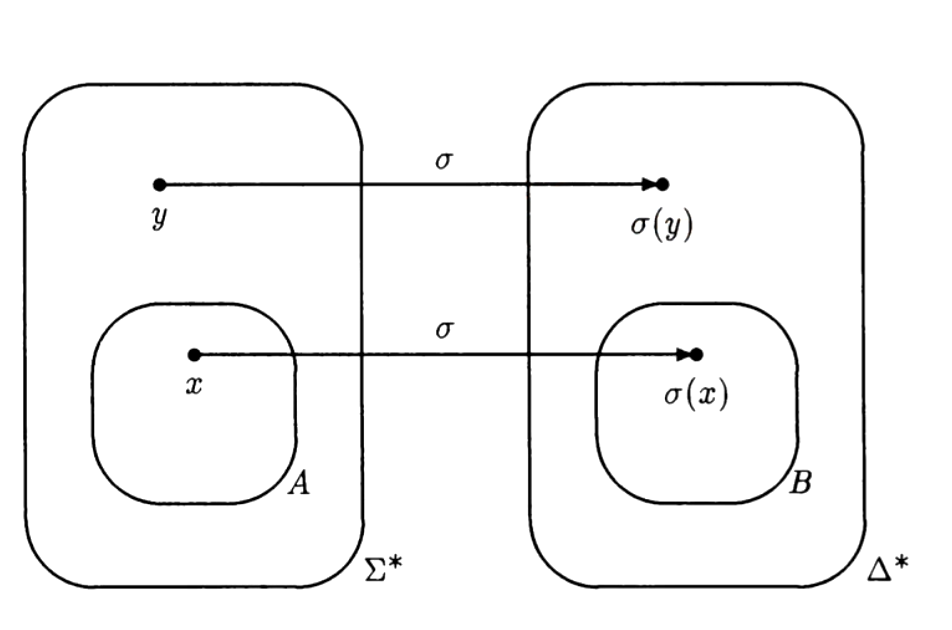
\includegraphics[width=0.6\textwidth]{eighteen.png}
	\caption{Mapping}
	\label{fig:eighteen-png}
\end{figure}
\end{tcolorbox}
\begin{tcolorbox}[colback=black!3!white,colframe=black!60!white,title=\begin{defn}Computability \label{Computability}\end{defn}]
The expression
\begin{align}
\sigma : \Sigma^{*} \to \Delta^{*}
\end{align}
Is a computable function if there is a decider that, on input $x$, halts with $\sigma(x)$ written on the tape.
\end{tcolorbox}
\begin{tcolorbox}[colback=black!3!white,colframe=black!60!white,title=\begin{defn}Reduction \label{Reduction}\end{defn}]
For $A \subseteq \Sigma^{*}$, $B \subseteq \Delta^{*}$ we say that $A \le_m B$ if there is a function  $\sigma : \Sigma^{*} \to \Delta^{*}$
\begin{enumerate}
	\item for all $x \in \Sigma^{*}, x \in A \iff \sigma(x) \in B$ 
	\item $\sigma$ is a computable function
\end{enumerate}
\end{tcolorbox}
\begin{tcolorbox}[colback=black!3!white,colframe=black!60!white,title=\begin{thm}Decidable \label{Decidable}\end{thm}]
	A language $L$ is decidable if and only if $L$ and $\overline{L}$ are both Turing-recognisable. 
		\begin{align}
		
		\end{align}
\end{tcolorbox}
\section{Revision}
\begin{figure}[H]
	\centering
	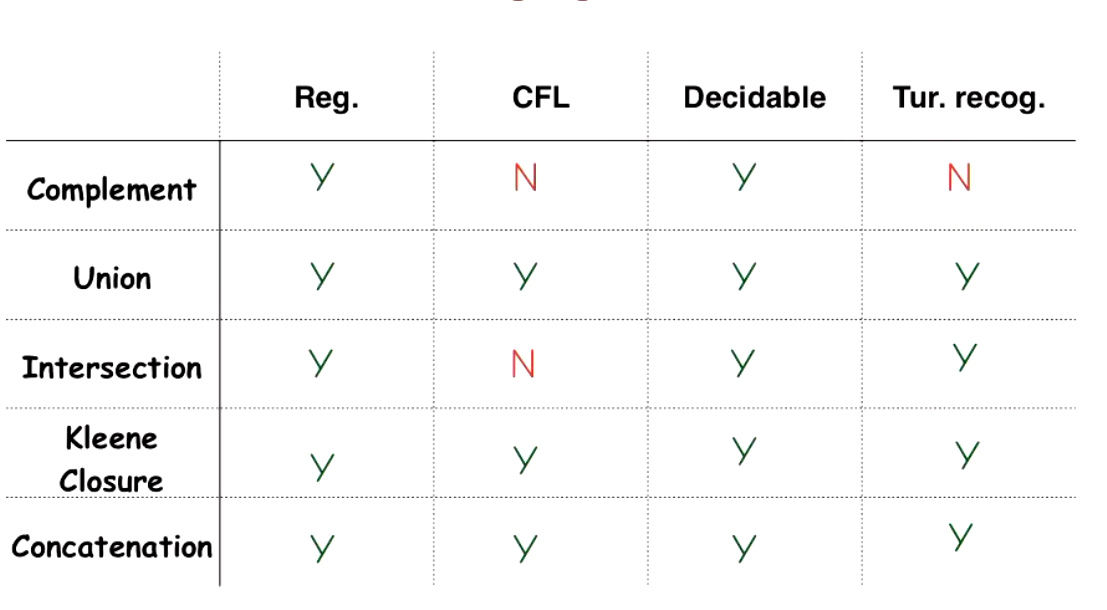
\includegraphics[width=0.8\textwidth]{table.png}
	\caption{Properties table: Closure}
	\label{fig:table-png}
\end{figure}
\begin{figure}[H]
	\centering
	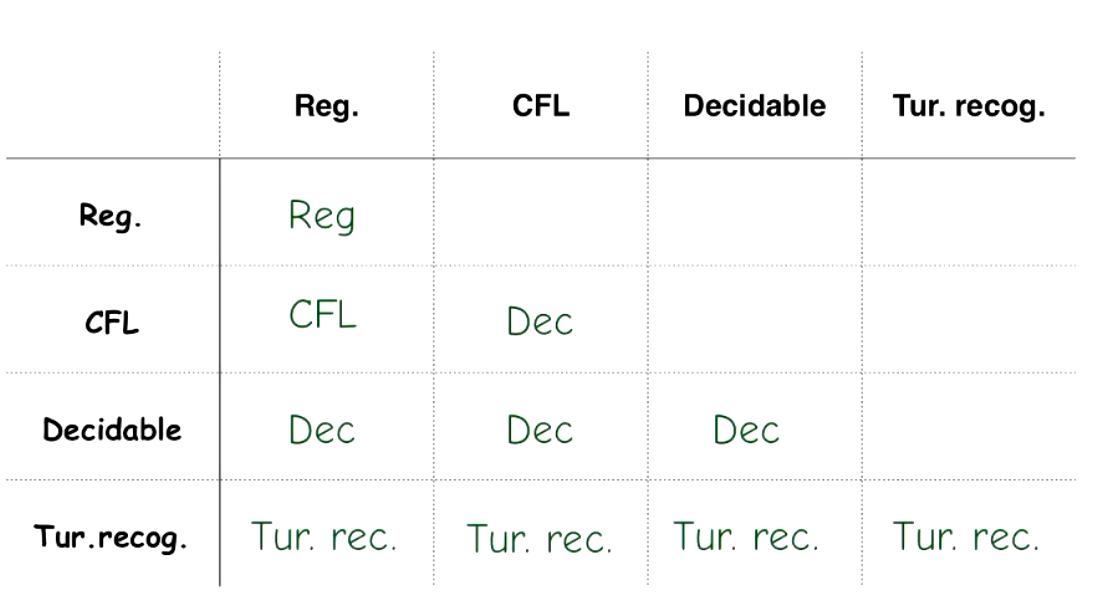
\includegraphics[width=0.8\textwidth]{pair.png}
	\caption{Pairwise closure: Intersection}
	\label{fig:pair-png}
\end{figure}
\end{document}
